\begin{bibunit}[apalike]

\setcounter{page}{1}


\begin{appendices}


%\section{Supplementary Figures}\label{secA}
\setcounter{figure}{0}
\renewcommand{\thefigure}{S\arabic{figure}}



%\begin{figure}[hbtp]
%    \centering
%    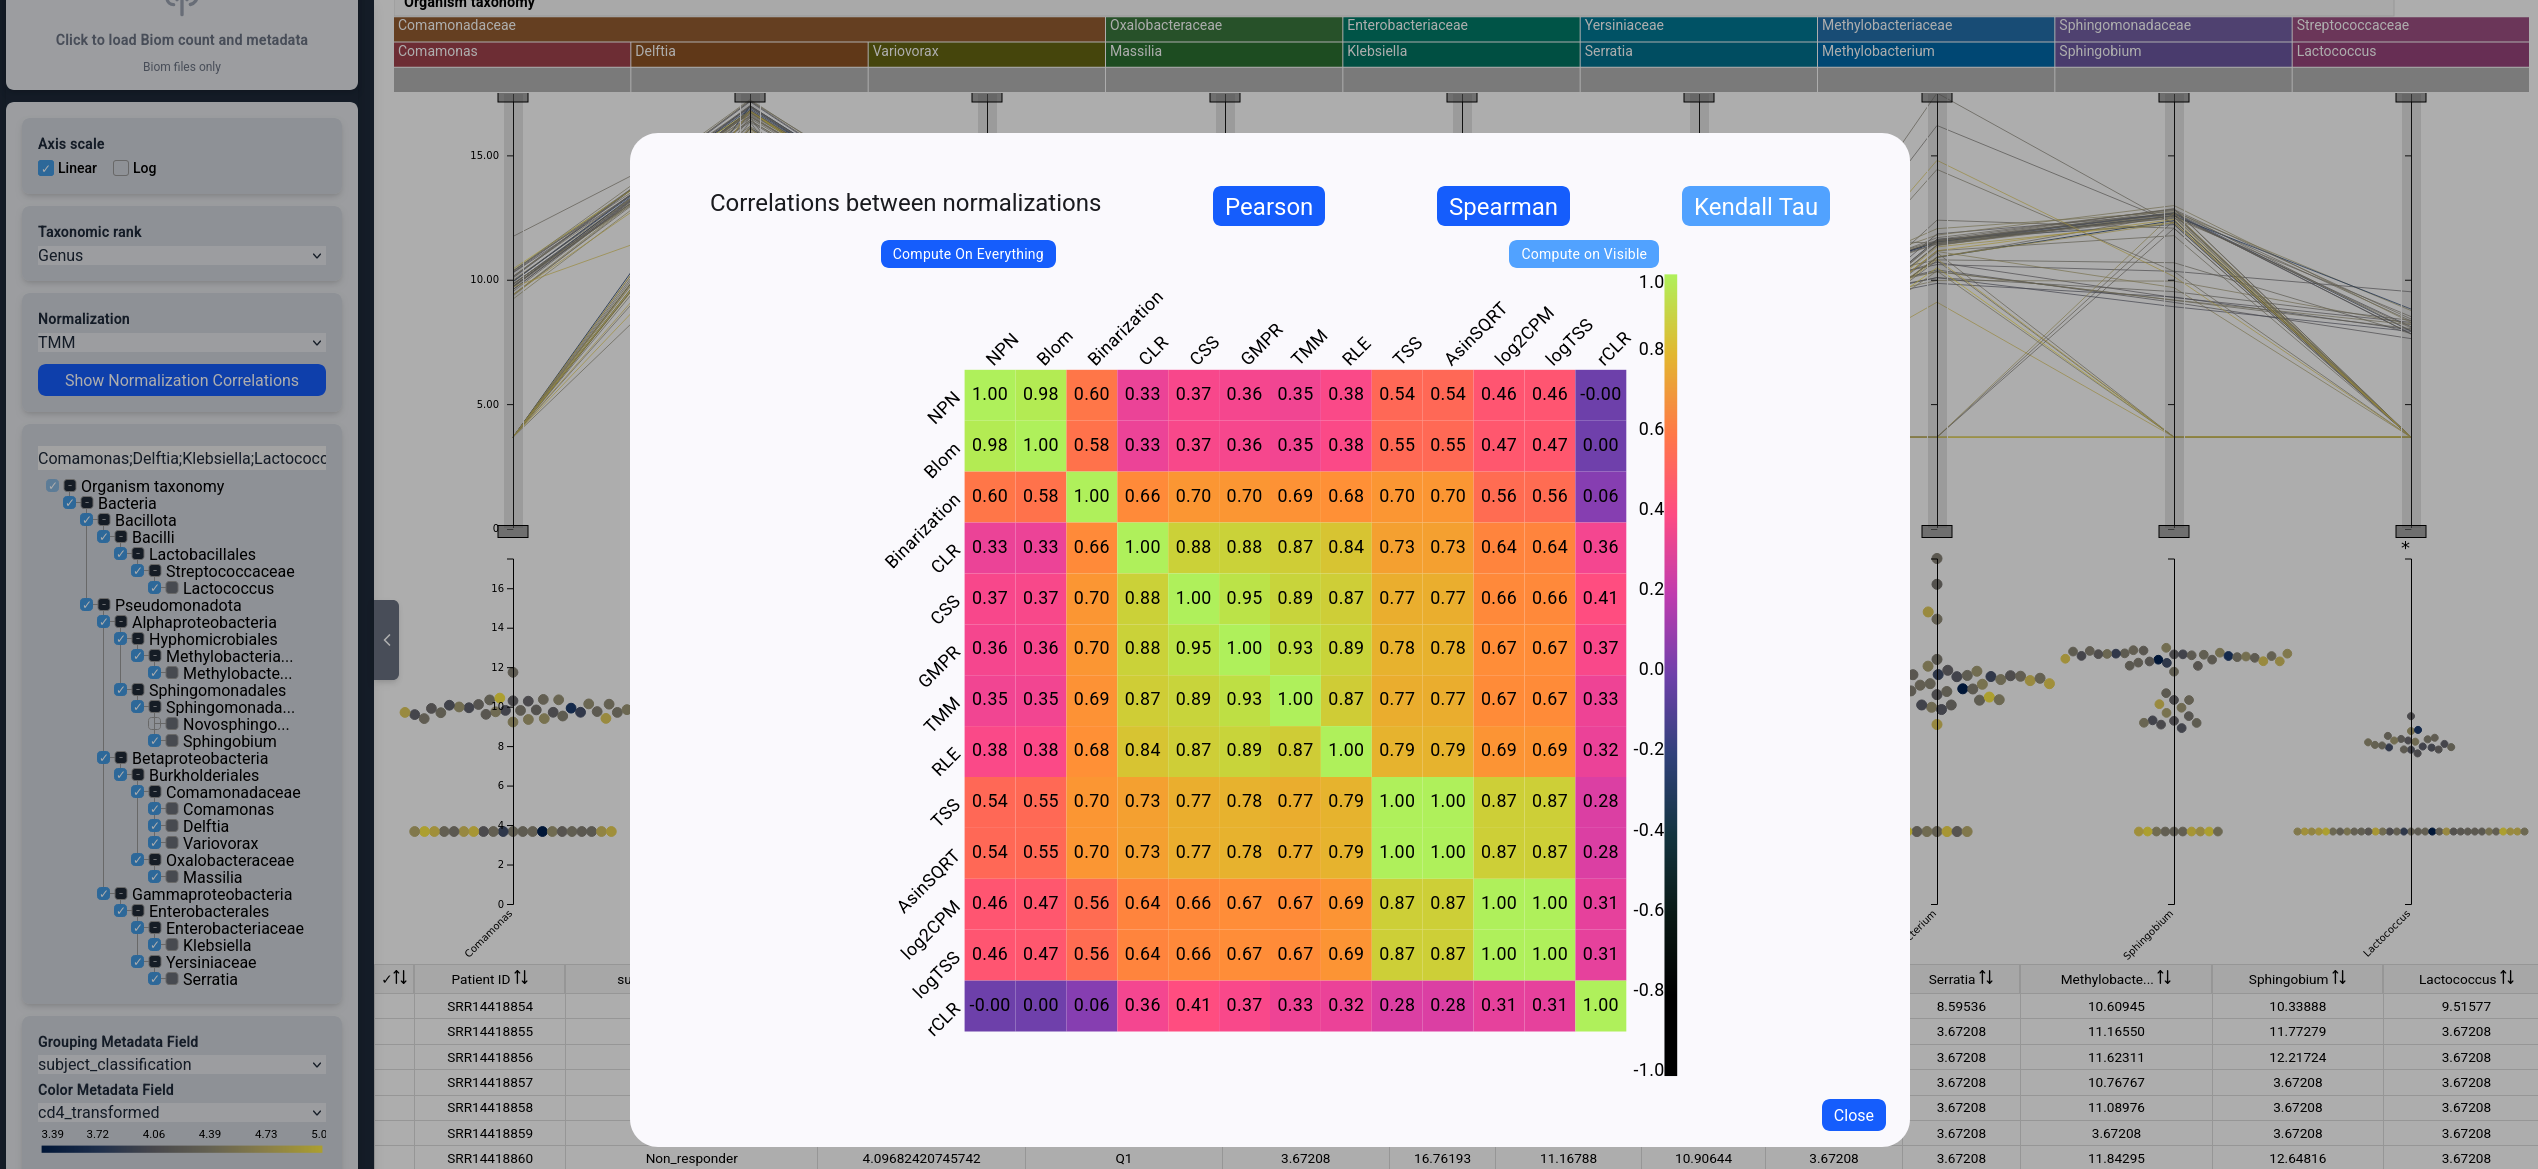
\includegraphics[width=\textwidth]{figures/v2/supp1.png}
%\caption{Comparison of normalization and transformation methods available in TaxaLoom for the Cleveland cohort, using the data presented in Figure~\ref{douek}. Pairwise correlations were computed between the vectorized abundance matrices obtained using each method. Similarity was evaluated using Kendall's correlation coefficient (shown), with Spearman's and Pearson's correlations also available through the interactive interface. Values closer to 1 indicate greater similarity between the abundance profiles obtained with the corresponding methods.}
%    \label{supp:cor_heatmap}
%\end{figure}


%\begin{figure}[htbp]
%    \centering
%    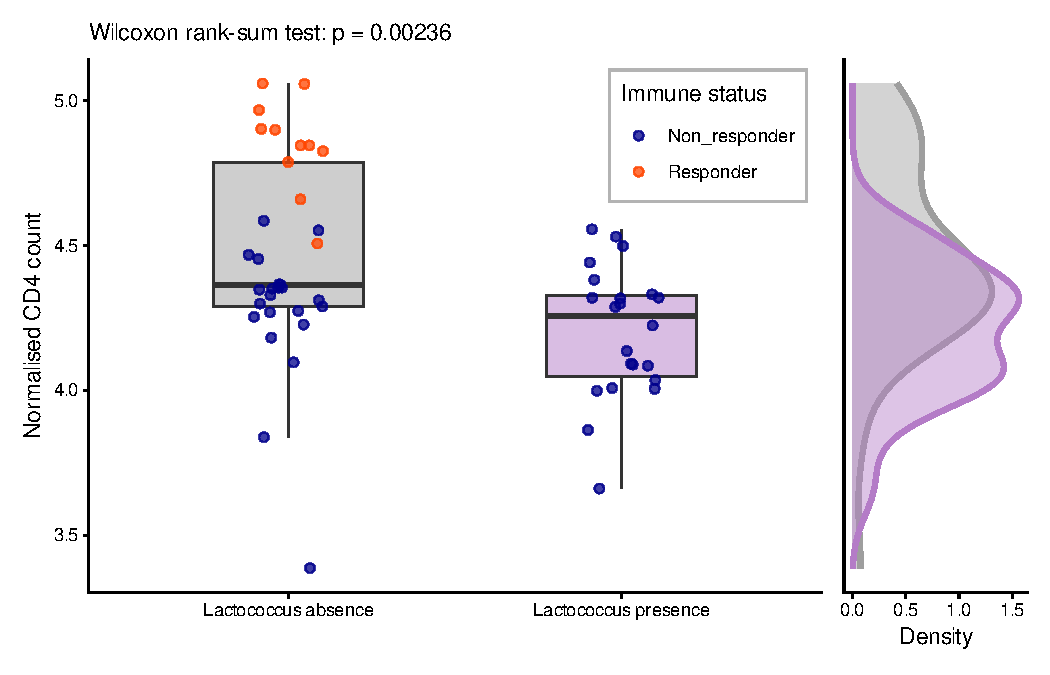
\includegraphics[width=\textwidth]{figures/supp1.pdf}
%    \caption{Boxplots of normalized CD4 T-cell counts according to \textit{Lactococcus} detection in the Cleveland cohort. Distribution of normalized CD4 T-cell counts in samples with and without detected \textit{Lactococcus}. Individual samples are coloured according to immune response status. Boxplots summarize the distribution within each group, with corresponding density distributions shown on the right. Normalized CD4 T-cell counts were significantly lower in samples with non-zero \textit{Lactococcus} abundance (Wilcoxon rank-sum test, $W=540.5$, $p=0.00236$).}    
%\label{figsupp:boxplots}
%\end{figure}



%\begin{figure}[htbp]
%    \centering
%    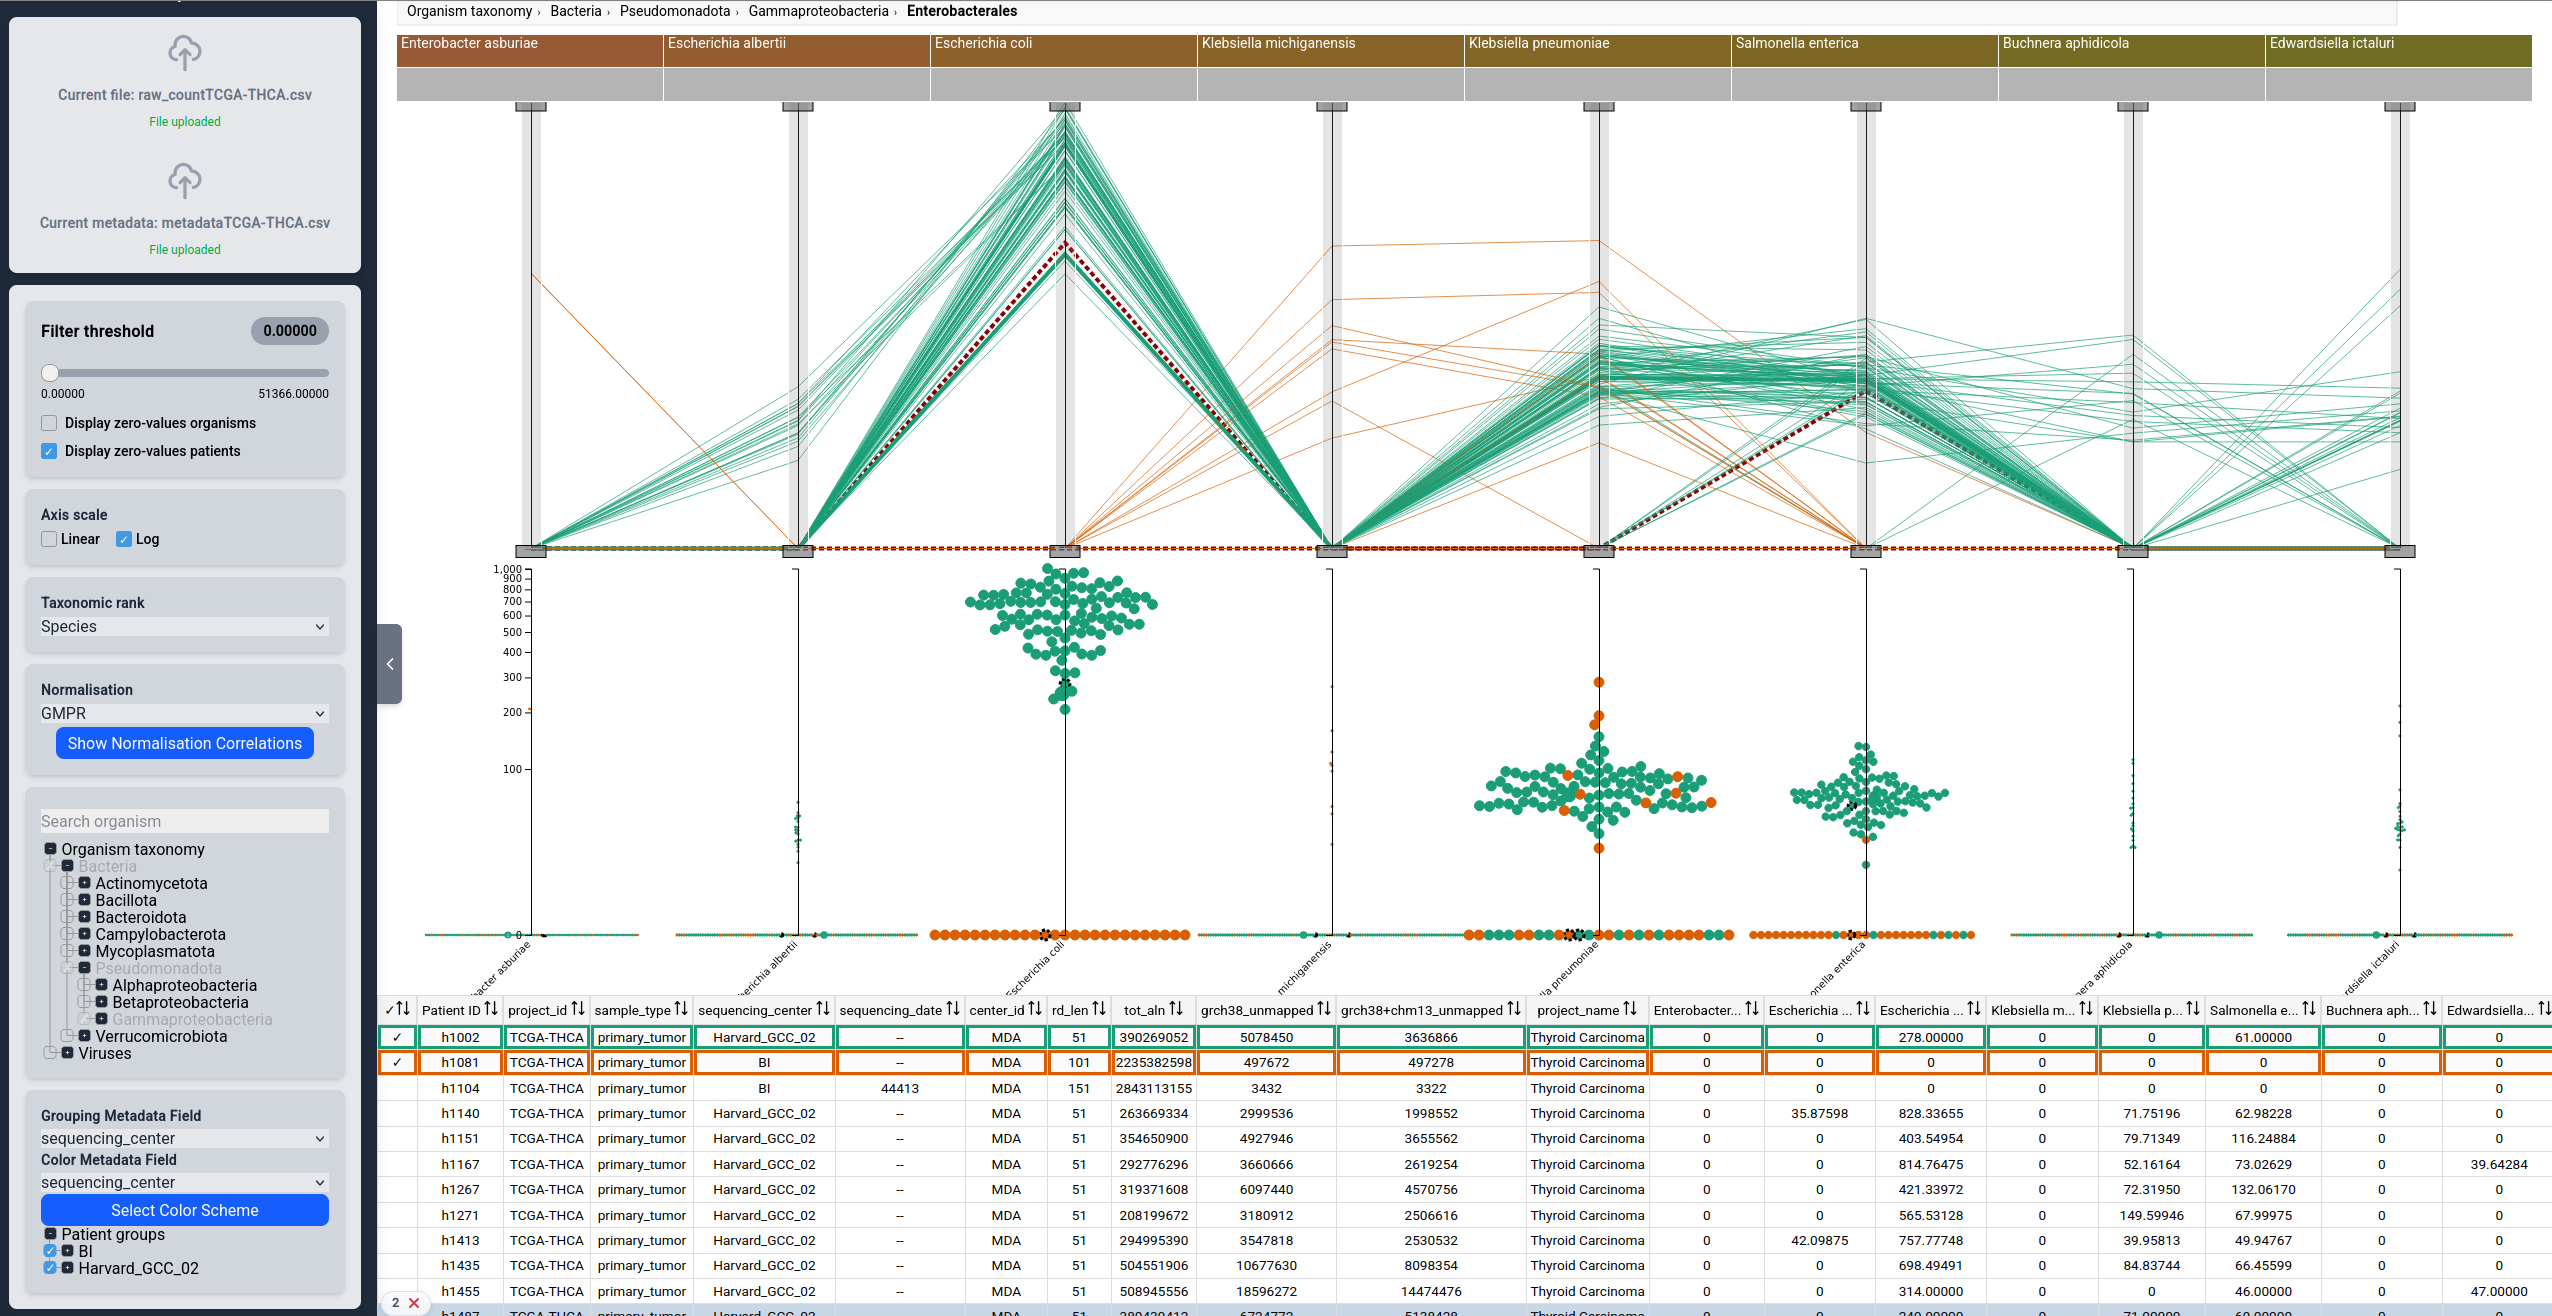
\includegraphics[width=\textwidth]{figures/supp3.png}
%    \caption{\textbf{Sample-level abundance profiles of Enterobacterales in TCGA-THCA.} TaxaLoom visualization restricted to species belonging to the order \textit{Enterobacterales} in the 98 TCGA-THCA \texttt{Primary Tumor} samples. Samples are coloured according to sequencing centre, allowing sequencing-associated abundance patterns to be identified across Enterobacterales species. Abundances were normalized using GMPR and displayed on a logarithmic scale.}
%    \label{figsupp:entero}
%\end{figure}

%\begin{figure}[htbp]
%    \centering
%    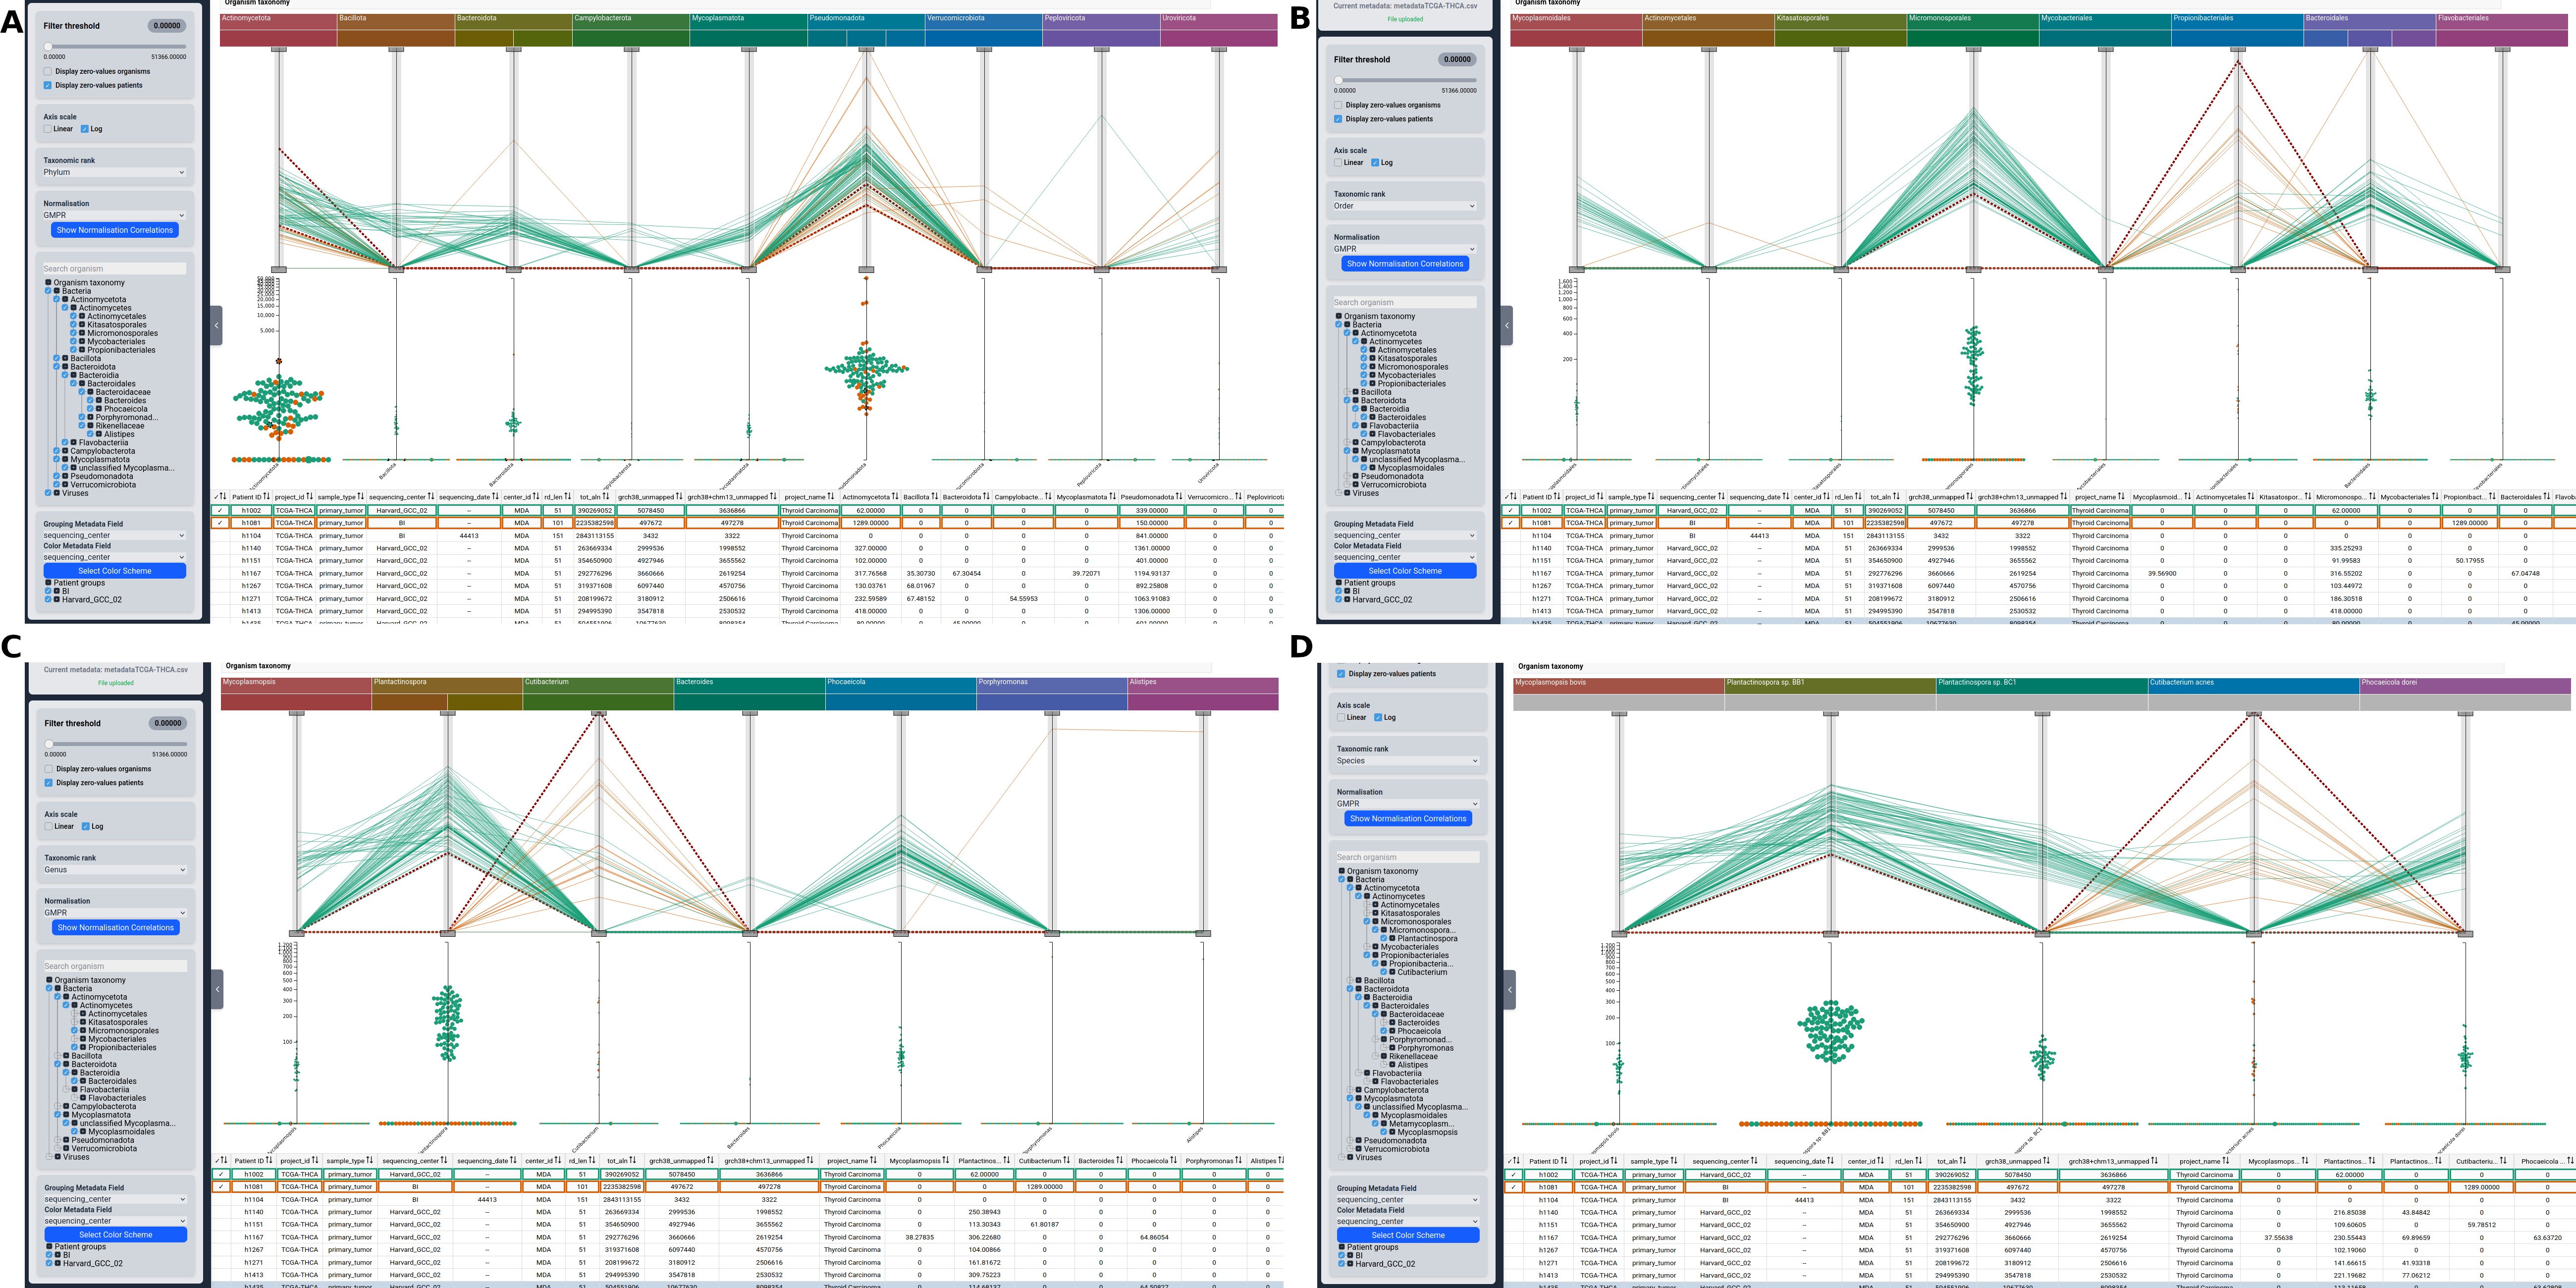
\includegraphics[width=\textwidth]{figures/supp2.png}
%    \caption{Progressive taxonomic filtering of TCGA-THCA microbial profiles using TaxaLoom. Taxonomic branches were successively filtered to focus on taxa exhibiting sequencing-associated abundance patterns. (\textbf{A}) Initial visualization at the phylum level. Selected phyla were removed to retain \textit{Actinomycetota}, \textit{Bacteroidota}, and \textit{Mycoplasmatota} for further exploration. (\textbf{B}) Resulting visualization at the order level, from which \textit{Mycoplasmoidales}, \textit{Micromonosporales}, \textit{Propionibacteriales}, and \textit{Bacteroidales} were retained. (\textbf{C}) Genus-level visualization, further restricted to \textit{Mycoplasmopsis}, \textit{Plantactinospora}, \textit{Cutibacterium}, and \textit{Phocaeicola}. (\textbf{D}) Final species-level visualization resulting from the successive taxonomic filtering. Abundances were normalized using GMPR and displayed on a logarithmic scale.}

%    \label{figsupp:conta_global}
%\end{figure}



\clearpage

\section{Supplementary Notes}

\subsection{Preprocessing methods available in TaxaLoom}\label{secA1}


Throughout this section, $y_{ji}$ and $q_{ji}$ denotes, respectively the raw and relative abundance of feature $i$ in sample $j$, and $N_j=\sum_{i=1}^{p}y_{ji}$ denotes the corresponding library size, where $p$ is the total number of features.

\subsubsection*{Binarisation}

Binarisation converts count data into presence-absence values by removing abundance information. Let $y_{ji}$ denote the raw count of feature $i$ in sample $j$.

The transformation is defined as

\[
x_{ji} =
\begin{cases}
1 & y_{ji} > 0 \\
0 & y_{ji} = 0
\end{cases}
\]

This transformation encodes only whether a feature is detected in a sample, disregarding quantitative abundance information.


\subsubsection*{Total Sum Scaling (TSS)}



Total sum scaling (TSS) transforms raw counts into relative abundances by normalizing each sample by its sequencing depth. Let $y_{ji}$ denote the raw count of feature $i$ in sample $j$.

The relative abundance is defined as

\[
q_{ji}=\frac{y_{ji}}{N_j}.
\]

which rescales each sample to sum to 1.


\subsubsection*{log2CPM}

log2 counts per million (log2CPM) rescales counts by library size and applies a $log_{2}$ transformation to stabilize the variance. Let $y_{ji}$ denote the raw count of feature $i$ in sample $j$.

The transformation is defined as

\[
x_{ji}=\log_2\left(\frac{y_{ji}+1}{N_j}\times10^6\right).
\]

where a pseudocount is added to avoid zeros before applying the log transform. It expresses counts as log-scaled counts per million reads, accounting for sequencing depth differences between samples.


\subsubsection*{TMM Normalisation}

TMM (Trimmed Mean of M-values) estimates a sample-specific scaling factor by comparing each sample to a reference sample \citep{robinson_scaling_2010}.

In the edgeR implementation, the reference sample $r$ is defined as the sample whose count-per-million upper quartile is closest to the mean upper quartile \citep{robinson_edger_2010}. For each feature $i$, an M-value representing the log-fold change between sample $j$ and the reference sample is computed as:

\[
M_{ji}=\log_{2}\left(\frac{y_{ji}/N_j}{y_{ri}/N_r}\right)
\]

where $y_{ji}$ and $y_{ri}$ denote the raw counts for feature $i$ in sample $j$ and reference sample $r$, respectively, and $N_j=\sum_i y_{ji}$ and $N_r=\sum_i y_{ri}$ are the corresponding library sizes.

An average abundance measure is also calculated as:
\[
A_{ji}=\frac{1}{2}\log_{2}\left(\frac{y_{ji}}{N_j}\cdot\frac{y_{ri}}{N_r}\right)
\]

The M- and A-values are then used to remove features with extreme fold changes or abundance values. Following the default TMM procedure, the 30\% highest and lowest M-values and the 5\% highest and lowest A-values are excluded \cite{robinson_scaling_2010}. The scaling factor is therefore estimated from features that are neither extreme in fold change nor in abundance.

The weight for feature $i$ and sample $j$ is defined as:

\[
w_{ji} = \frac{N_j - y_{ji}}{N_j \cdot y_{ji}} + \frac{N_r - y_{ri}}{N_r \cdot y_{ri}}
\]
The TMM scaling factor for sample $j$ relative to the reference is then obtained from the weighted mean of the M-values retained after trimming:

\[
\log_2(s_j)=\frac{\sum_{i \in \mathcal{I}} w_{ji} M_{ji}}{\sum_{i \in \mathcal{I}} w_{ji}},
\]

where $\mathcal{I}$ denotes the set of features retained after M- and A-value trimming. The resulting normalization factors $s_j$ are rescaled so that their product across samples equals one \citep{robinson_edger_2010}. As for RLE normalization, the effective library size is then obtained as:

\[
N_j^{*}=N_j s_j,
\]

where $N_j$ is the original library size of sample $j$.



\subsubsection*{RLE normalisation}

Relative log expression (RLE) normalization estimates sample-specific scaling factors using the median-ratio method proposed in \citep{anders_differential_2010}. For each feature $i$, the geometric mean of its counts across all $n$ samples is calculated:

$$
g_i=\left(\prod_{j=1}^{n}y_{ji}\right)^{1/n},
$$

where $y_{ji}$ denotes the raw count for feature $i$ in sample $j$. The resulting values $g_i$ define a reference abundance profile against which each sample is compared. The scaling factor $s_j$ for each sample is then calculated as the median of the ratios between its feature counts and the corresponding reference values:

$$
f_j={\operatorname{median}}\left(\frac{y_{ji}}{g_i}\right).
$$

In the edgeR implementation, these factors are rescaled so that their product across samples equals one \citep{robinson_edger_2010}. The resulting normalization factor $s_j$ is used to calculate the effective library size of sample $j$:

$$
N_j^{*}=N_j s_j,
$$

where $N_j$ is the original library size of sample $j$.





\subsubsection*{Blom transform}


The Blom transformation converts abundance values into rank-based normal scores \cite{blom_statistical_1958}. For each feature $i$, abundance values are first ranked across the $n$ samples. The rank $r_{ji}$ of feature $i$ in sample $j$ is then converted into a value between 0 and 1:


\[
q_{ji}=\frac{r_{ji}-3/8}{n+1/4},
\]
where $n$ is the number of samples. The resulting value $q_{ji}$ is then mapped to the corresponding quantile of the standard normal distribution using its inverse cumulative distribution function:

\[
x_{ji}=\Phi^{-1}(q_{ji}),
\]

where $\Phi^{-1}(\cdot)$ denotes the inverse cumulative distribution function of a normal distribution with mean 0 and standard deviation 1. The resulting $x_{ji}$ values are therefore rank-based normal scores that approximate a standard normal distribution while preserving the ordering of the original abundance values.


\subsubsection*{NPN transform}

The non-paranormal (NPN) transformation uses a rank-based Gaussianization procedure \citep{liu_nonparanormal_2009}. For each feature $i$, abundance values are ranked across the $n$ samples. The rank $r_{ji}$ of feature $i$ in sample $j$ is first mapped to a value between 0 and 1:

\[
q_{ji} = \frac{r_{ji}}{n+1},
\]

where $n$ is the number of samples.

These values are then transformed using the inverse cumulative distribution function of the standard normal distribution:

\[
x_{ji} = \Phi^{-1}(q_{ji}),
\]

yielding rank-based values that approximately follow a normal distribution.

In practice, a truncated version of the NPN transformation was used, as implemented in the \textit{huge} R package \citep{zhao_huge_2012}. Before applying the inverse normal transformation, values at the lower and upper extremes are constrained to predefined limits. This truncation prevents extreme ranks from producing excessively large positive or negative transformed values.

\subsubsection*{GMPR transform}

GMPR (Geometric Mean of Pairwise Ratios), as implemented in the \textit{MicrobiomeStat} R package, is a size-factor-based normalization method designed for sparse count data \cite{chen_gmpr_2018}.

For each pair of samples $(j,k)$, abundance ratios are calculated using only features that are non-zero in both samples. A pairwise ratio is defined as the median of these ratios:
\[
r_{jk} = \operatorname{median}_{i \in \mathcal{I}_{jk}} \left( \frac{y_{ji}}{y_{ki}} \right),
\]
where $\mathcal{I}_{jk} = \{i:y_{ji}>0,\;y_{ki}>0\}$ denotes the set of shared non-zero features between samples $j$ and $k$.

For each sample $j$, a sample-specific scaling factor $s_j$ is then calculated as the geometric mean of its pairwise ratios with the other samples:
\[
s_j = \left( \prod_{k \neq j} r_{jk} \right)^{\frac{1}{n}},
\]


where $n$ is the number of samples. The resulting scaling factor summarizes the abundance of sample $j$ relative to the other samples while reducing the influence of zeros by considering only features detected in both samples.

Normalized abundances are then obtained by dividing the raw counts by the corresponding scaling factor:

\[
x_{ji} = \frac{y_{ji}}{s_j}.
\]

\subsubsection*{CSS transform}

Cumulative sum scaling (CSS), implemented in the \textit{metagenomeSeq} R package, is a normalization method designed for sparse microbiome count data \citep{paulson_differential_2013}.

CSS determines a percentile of the count distribution from the data, above which highly abundant features are excluded from the calculation of the scaling factor. For each sample $j$, the scaling factor $s_j$ is then calculated as the cumulative sum of counts up to the selected percentile:

$$
s_j=\sum_{i:\,y_{ji}\le q_{\hat l}(y_j)}y_{ji},
$$

where $q_{\hat l}(y_j)$ denotes the count value corresponding to the selected percentile in sample $j$.

Normalized abundances are obtained by dividing each raw count by the corresponding scaling factor:

$$
x_{ji}=\frac{y_{ji}}{s_j}.
$$

By calculating the scaling factor without the most highly abundant features, CSS reduces their influence on the normalization.


\subsubsection*{AsinSquareRoot}

The arcsine square-root transformation is applied to relative abundance data to stabilize variance, particularly for proportions close to 0 or 1. Let $q_{ji}$ denote the relative abundance of feature $i$ in sample $j$, obtained after total sum scaling.

The transformation is defined as

\[
x_{ji} = \arcsin\left(\sqrt{q_{ji}}\right),
\]

The transformation reduces the dependence of the variance on the mean that is characteristic of proportional data, producing values with a more stable variance across the range of relative abundances.

\subsubsection*{CLR transform}

The centered log-ratio (CLR) transformation maps relative abundances to a log-ratio scale relative to the geometric mean of all features within a sample \citep{aitchison_statistical_1982}. Let $g_j$ denote the geometric mean of the relative abundances in sample $j$.

The transformation is defined as:

\[
x_{ji} = \ln\left(\frac{q_{ji}}{g_j}\right),
\]

where

\[
g_j = \left(\prod_{k=1}^{p} q_{jk}\right)^{1/p},
\]

and $p$ is the total number of features. The resulting values express the abundance of each feature relative to the geometric mean abundance of all features within the same sample.

\subsubsection*{rCLR transform}

The robust centered log-ratio (rCLR) transformation is a modification of the CLR transformation that accommodates zero values by calculating the geometric mean using only non-zero features \citep{martino_novel_2019}.

For each sample $j$, the geometric mean is calculated using only non-zero relative abundances:

\[
g_j=\exp\left(\frac{1}{m_j^{+}}\sum_{k:q_{jk}>0}\ln(q_{jk})\right),
\]

where $m_j^{+}$ denotes the number of non-zero features in sample $j$.

The rCLR transformation is then defined as:

\[
x_{ji}=
\begin{cases}
\ln\left(\frac{q_{ji}}{g_j}\right) & q_{ji}>0,\\
0 & q_{ji}=0.
\end{cases}
\]

The resulting values express each non-zero feature as a log-ratio relative to the geometric mean of the non-zero features within the same sample, while zero values remain zero in the transformed data.


\subsection{Microbial abundance filtering}\label{secA2}

Both datasets used in the case studies were derived from host-dominated sequencing data and we therefore add an additional filtering step before their use in TaxaLoom. The Cleveland cohort was generated from total-RNA sequencing of blood samples, in which human-derived reads represented the majority of the sequencing data \cite{nganou-makamdop_translocated_2021,colajanni_benchmarking_2026}. Similarly, the TCGA microbial profiles were obtained from the reanalysis of human whole-genome sequencing (WGS) data \citep{ge_comprehensive_2025}. As the microbial signal represents only a small fraction of these datasets, we applied dataset-specific filtering procedures to reduce low-abundance and potentially spurious taxonomic classifications before visualization. 

We used a similar strategy for both dataset as they were reanalysed using similar procedure. 

\subsubsection*{Cleveland cohort filtering} \label{secA3}

The Cleveland cohort, originally described by \citet{lederman_immunologic_2011} and subsequently sequenced and analysed by \citet{nganou-makamdop_translocated_2021}, comprised 55 HIV-infected individuals receiving combined antiretroviral therapy (cART). Participants were classified as immune responders ($n=11$) or immune non-responders ($n=44$) based on CD4+ T-cell counts above 500 or below 350 cells/$\mu$L, respectively, after at least 24 months of virologic suppression on cART \citep{lederman_immunologic_2011}. Individual CD4+ T-cell counts were also available, providing both categorical immune response status and a quantitative measure of immune recovery.

Raw sequencing data were retrieved from the Sequence Read Archive (SRA) and reanalysed as described in our previous benchmarking study \citep{colajanni_benchmarking_2026}. The resulting genus-level raw count data were retrieved from this study, while the associated clinical metadata were obtained from \citet{nganou-makamdop_translocated_2021}.

CD4+ T-cell counts were log-transformed to facilitate visualization.

Following taxonomic classification, genera considered biologically implausible in human blood were manually excluded based on their known host range and ecology. This filtering removed 23 genera, including plant-associated viruses and pathogens: \textit{Orthotospovirus} \citep{kormelink_bunyavirales_2021}, \textit{Albugo} \citep{kemen_gene_2011}, \textit{Phytophthora} \citep{meng_phytophthora_2014}, \textit{Entyloma} \citep{kruse_broad_2018}, \textit{Sporisorium} \citep{zhao_sporisorium_2022}, \textit{Stenocarpella} \citep{health_plh_pest_2022}, \textit{Sclerotinia} \citep{derbyshire_evolutionary_2022}, \textit{Taphrina} \citep{nigon_exploring_2026}, and \textit{Zymoseptoria} \citep{quaedvlieg_zymoseptoria_2011}. Genera associated with highly specific non-human or environmental niches were also removed, including the bee gut symbiont \textit{Gilliamella} \citep{kwong_evolution_2015}; the haloarchaea \textit{Halobacterium} and \textit{Haloplanus} \citep{fendrihan_extremely_2006}, \textit{Halorubrum} and \textit{Natronomonas} \citep{kamekura_diversity_1998}, and \textit{Natrinema} \citep{strakova_natrinema_2023}; the wood- or tree-associated fungi \textit{Hornodermoporus} \citep{yuan_species_2023}, \textit{Chrysoporthe} \citep{van_der_nest_ima_2021}, \textit{Immersiporthe} \citep{chen_serious_2013}, and \textit{Phlebiopsis} \citep{iwata_omics_2021}; the mushroom-forming genus \textit{Entoloma} \citep{liu_additions_2025}; the insect-parasitic nematode \textit{Hexamermis} \citep{poinar_hexamermis_1985,lee_hexamermis_2026}; and the dung-associated fungus \textit{Sordaria} \citep{newcombe_revisiting_2016}. Finally, \textit{Sinsheimervirus} was excluded because this genus contains PhiX174, which is commonly used as an Illumina sequencing control \citep{illumina_phix_control}. 

To reduce low-abundance taxonomic assignments, read-count cutoffs ranging from 1 to 50 reads were evaluated independently for each sample. For each cutoff, taxa with fewer reads were considered absent and their counts were set to zero. The resulting relationship between the minimum abundance required for detection and the number of taxa remaining in each sample is shown in Figure~\ref{figsuppsupp}.

A sample-specific cutoff was selected as the first point at which the mean relative decrease in the number of taxa reached 5\% over a sliding window of five consecutive values. This criterion was designed to identify the beginning of a plateau, beyond which increasing the cutoff produced relatively little change in the number of detected taxa, thereby limiting low-abundance classifications potentially resulting from spurious taxonomic assignments.

\begin{figure}[htbp]
\centering
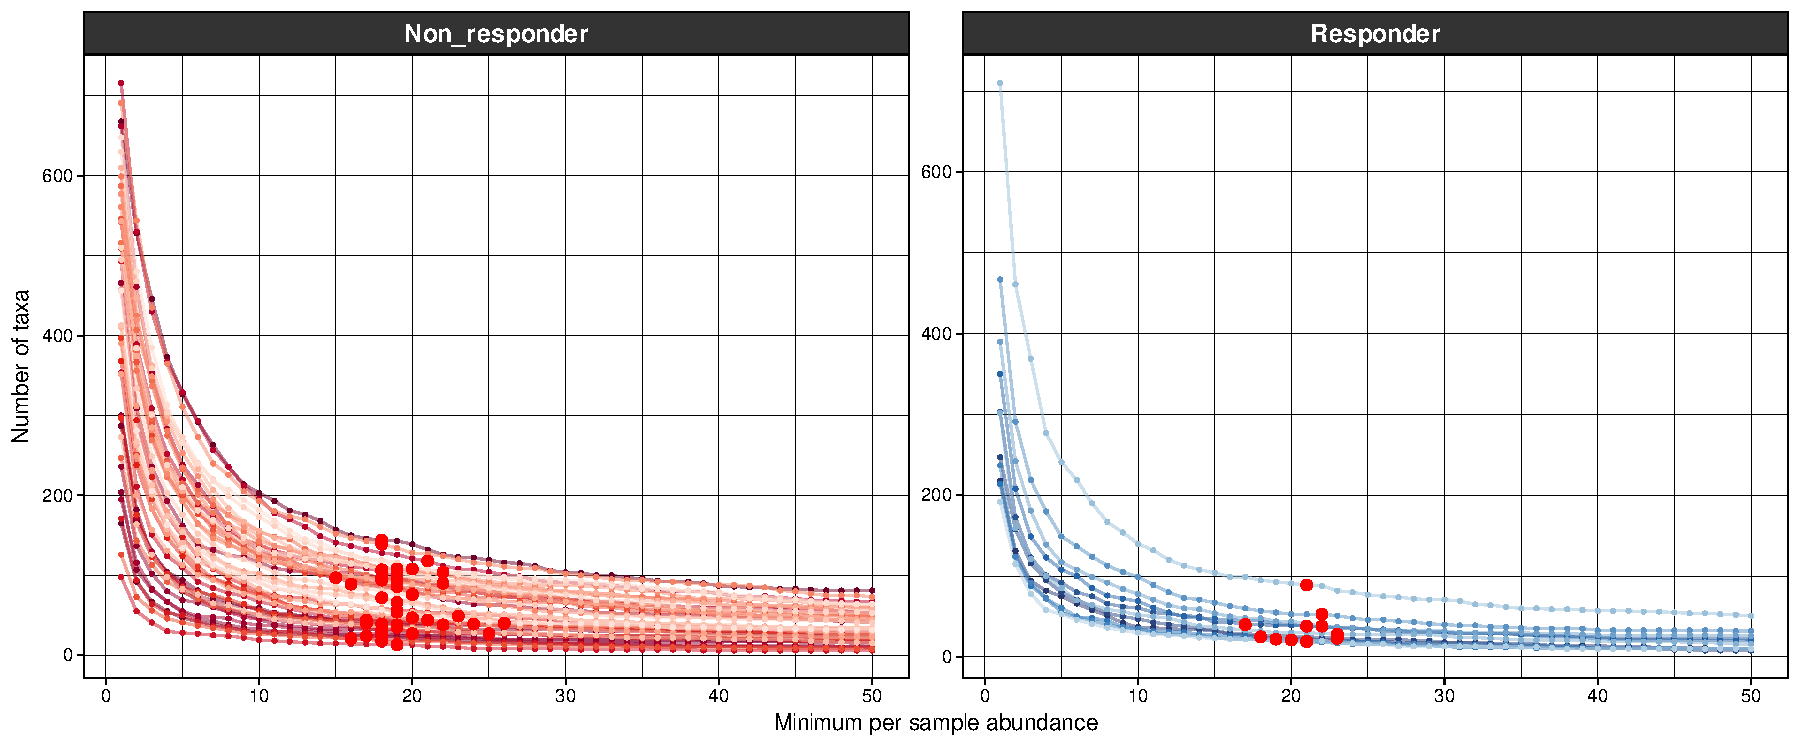
\includegraphics[width=\textwidth]{figures/supp_fig_filtration_cleveland.pdf}
\caption{Sample-specific abundance filtering for the Cleveland cohort. Number of taxa retained in each sample as a function of the minimum read-count threshold required to consider a taxon present. Taxa with counts below the corresponding threshold were considered absent and their counts were set to zero. Red points indicate the threshold selected independently for each sample, defined as the first point at which the mean relative decrease in the number of retained taxa reached 5\% over a sliding window of five consecutive thresholds.}
\label{figsuppsupp}
\end{figure}

For the case application, we focused on the 29 bacterial genera previously reported as differentially abundant between immune responders and immune non-responders by \citet{nganou-makamdop_translocated_2021}: \textit{Mycobacterium}, \textit{Kocuria}, \textit{Microbacterium}, \textit{Lactococcus}, \textit{Hymenobacter}, \textit{Sphingobacterium}, \textit{Xanthomonas}, \textit{Serratia}, \textit{Klebsiella}, \textit{Achromobacter}, \textit{Comamonas}, \textit{Hydrogenophaga}, \textit{Acidovorax}, \textit{Variovorax}, \textit{Ramlibacter}, \textit{Delftia}, \textit{Roseateles}, \textit{Rhizobacter}, \textit{Rubrivivax}, \textit{Massilia}, \textit{Burkholderia}, \textit{Ralstonia}, \textit{Methylophilus}, \textit{Sphingobium}, \textit{Novosphingobium}, \textit{Ochrobactrum}, \textit{Methylobacterium}, \textit{Brevundimonas}, and \textit{Rickettsia}.

Prior to visualization, genera detected in fewer than 22 of the 55 samples (40\% prevalence) were excluded to reduce sparsity. The remaining abundance counts were normalized using the trimmed mean of M-values (TMM) method. Within TaxaLoom, genera were further filtered using the built-in Wilcoxon rank-sum test, retaining those with a nominal $p<0.05$. This resulted in 9 genera selected for visualization: \textit{Lactococcus}, \textit{Serratia}, \textit{Klebsiella}, \textit{Comamonas}, \textit{Variovorax}, \textit{Delftia}, \textit{Massilia}, \textit{Sphingobium}, and \textit{Methylobacterium}.


\subsubsection*{TCGA-THCA filtering} \label{secA4}

Reanalysed TCGA microbial abundance data and associated metadata were obtained from \citet{ge_comprehensive_2025}. The complete dataset comprised 5,734 whole-genome sequencing samples and 11,389 detected species. Complete taxonomic lineages were reconstructed from the taxonomic identifiers provided in the dataset using TaxonKit \citep{shen_taxonkit_2021}. Samples with fewer than 1,000 total microbial counts were excluded to ensure sufficient microbial signal for subsequent exploration.

For the technical case application, the analysis was restricted to TCGA thyroid carcinoma (TCGA-THCA). The complete TCGA dataset was too large for practical interactive exploration with TaxaLoom, while the objective of this case application was to investigate technical covariates rather than cancer-specific abundance patterns. TCGA-THCA was selected because it contained a large number of \texttt{Primary Tumor} samples from both sequencing centres while remaining sufficiently small for efficient exploration. The resulting dataset comprised 122 \texttt{Primary Tumor} samples, including 26 from \texttt{BI} and 96 from \texttt{Harvard\_GCC\_02}.

To further reduce low-abundance taxonomic assignments within the retained samples, sample-specific abundance cutoffs ranging from 1 to 250 counts were evaluated independently for each sample. For each cutoff, species with counts below the threshold were considered absent and their counts were set to zero. The selected cutoff corresponded to the first point at which the mean relative decrease in the number of retained taxa fell below 1\% over a sliding window of five consecutive cutoff values (Figure~\ref{figsuppsupp2}). The wider range of candidate cutoffs and more stringent plateau criterion compared with the Cleveland cohort were used to accommodate the greater heterogeneity in microbial abundance observed across the TCGA samples.


\begin{figure}[htbp]
\centering
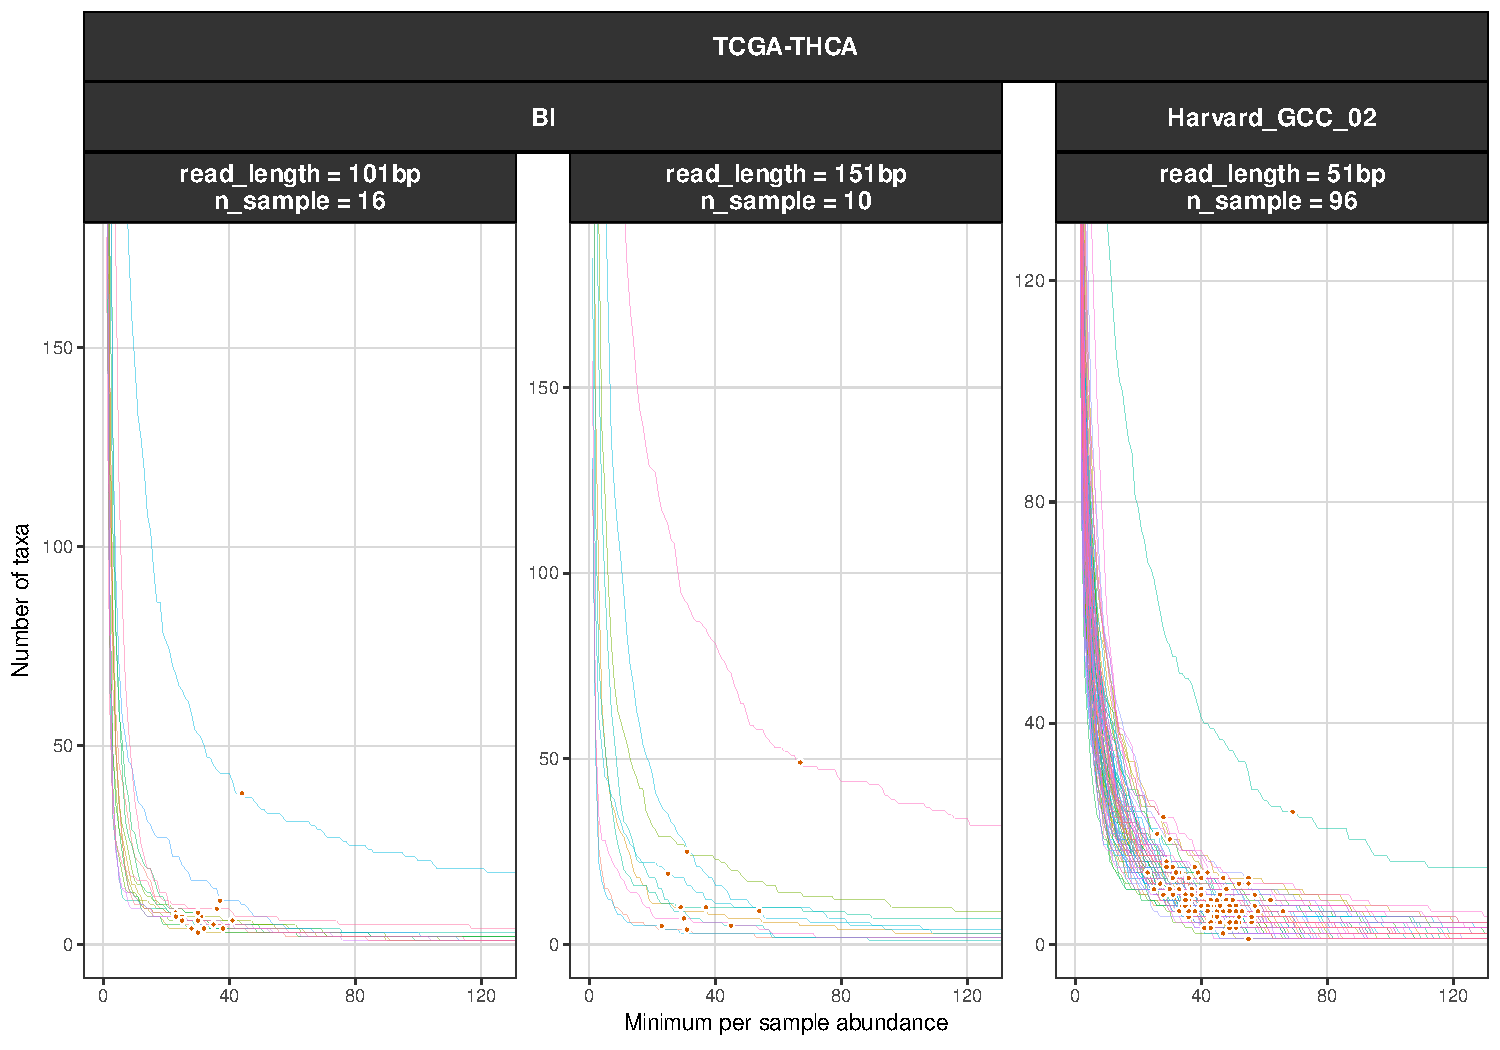
\includegraphics[width=\textwidth]{figures/supp_filtration_THCA.pdf}
\caption{Sample-specific abundance filtering for the TCGA-THCA, primary tumor samples. Number of taxa retained in each sample as a function of the minimum read-count threshold required to consider a taxon present. Taxa with counts below the corresponding threshold were considered absent and their counts were set to zero. Red points indicate the threshold selected independently for each sample, defined as the first point at which the mean relative decrease in the number of retained taxa reached 1\% over a sliding window of five consecutive thresholds.}
\label{figsuppsupp2}
\end{figure}


\newpage


\putbib[sn-bibliography]

\end{appendices}




\end{bibunit}